\section{Tính đơn điệu và cực trị của hàm số}
\subsection{Đề 1}
\caulc
\Opensolutionfile{ans}[ans/ans-2-B1-De1]
%%%==============EX_1============%%%
\begin{ex}%[2D1H1-2]
	Cho hàm số $y=f(x)$ xác định trên $\mathbb{R}$ và có bảng biến thiên như hình vẽ sau
	\begin{center}
		
\begin{tikzpicture}
			\tkzTabInit[nocadre=false,lgt=2,espcl=2,deltacl=0.5]
			{$x$/1 , $f'(x)$/1 , $f(x)$/2}
			{$-\infty$,$0$,$1$,$+\infty$}
			\tkzTabLine{,-,0,+,0,-,}
			\tkzTabVar{+/$+\infty$,-/$-1$,+/$0$,-/$-\infty$}
		\end{tikzpicture}
	\end{center}
	Hàm số đồng biến trên khoảng nào trong các khoảng sau đây?
	\choice
	{\True $(0; 1)$}
	{$(-\infty; 0)$}
	{$(1;+\infty)$}
	{$(0;+\infty)$}
	\loigiai{
		Hàm số đồng biến trên khoảng $(0; 1)$.
	}
\end{ex}
%%%==============EX_2============%%%
\begin{ex}%[2D1N1-2]
	Cho hàm số $y=f(x)$ xác định trên $\mathbb{R}$ và có bảng biến thiên như hình vẽ sau
\begin{center}
	
\begin{tikzpicture}
		\tkzTabInit[nocadre=false,lgt=2,espcl=2,deltacl=0.5]
		{$x$/1 , $f'(x)$/1 , $f(x)$/2}
		{$-\infty$,$2$,$6$,$+\infty$}
		\tkzTabLine{,+,0,-,0,+,}
		\tkzTabVar{-/$-\infty$,+/$10$,-/$0$,+/$+\infty$}
	\end{tikzpicture}
\end{center}
	Hàm số nghịch biến trên khoảng nào trong các khoảng sau đây?
	\choice
	{$(-\infty; 2)$}
	{$(6;+\infty)$}
	{\True $(2; 6)$}
	{$(-\infty; 6)$}
	\loigiai{
		Hàm số nghịch biến trên khoảng $(2;6)$.
	}
\end{ex}
%%%==============EX_3============%%%
\begin{ex}%[2D1H2-2]
	Cho hàm số $y=f(x)$ xác định trên $\mathbb{R}$ và có bảng biến thiên như hình vẽ sau
	\begin{center}
		\begin{center}
			
\begin{tikzpicture}
				\tkzTabInit[nocadre=false,lgt=2,espcl=2,deltacl=0.5]
				{$x$/1 , $f'(x)$/1 , $f(x)$/2}
				{$-\infty$,$6$,$11$,$+\infty$}
				\tkzTabLine{,+,0,-,0,+,}
				\tkzTabVar{-/$-\infty$,+/$-10$,-/$-20$,+/$+\infty$}
			\end{tikzpicture}
		\end{center}
	\end{center}
	Tìm điểm cực tiểu của hàm số $y=f(x)$.
	\choice
	{$x=-10$}
	{\True $x=11$}
	{$x=6$}
	{$x=-20$}
	\loigiai{
		Điểm cực tiểu của hàm số $y=f(x)$ là $x=11$.
	}
\end{ex}
%%%==============EX_4============%%%
\begin{ex}%[2D1H2-2]
	Cho hàm số $y=f(x)$ xác định trên $\mathbb{R}$ và có bảng biến thiên như hình vẽ sau.
	\begin{center}
		
\begin{tikzpicture}
			\tkzTabInit[nocadre=false,lgt=2,espcl=2,deltacl=0.5]
			{$x$/1 , $f'(x)$/1 , $f(x)$/2}
			{$-\infty$,$8$,$9$,$+\infty$}
			\tkzTabLine{,+,0,-,0,+,}
			\tkzTabVar{-/$-\infty$,+/$-8$,-/$-17$,+/$+\infty$}
		\end{tikzpicture}
	\end{center}
	Tìm điểm cực đại của hàm số $y=f(x)$.
	\choice
	{$x=-8$}
	{$x=-17$}
	{$x=9$}
	{\True $x=8$}
	\loigiai{
		Điểm cực đại của hàm số  là $x=8$.
	}
\end{ex}
%%%==============EX_5============%%%
\begin{ex}%[2D1H2-2]
	Cho hàm số $y=f(x)$ xác định trên $\mathbb{R}$ và có bảng biến thiên như hình vẽ sau.
		\begin{center}
		
\begin{tikzpicture}
			\tkzTabInit[nocadre=false,lgt=2,espcl=2,deltacl=0.5]
			{$x$/1 , $f'(x)$/1 , $f(x)$/2}
			{$-\infty$,$9$,$10$,$+\infty$}
			\tkzTabLine{,-,0,+,0,-,}
			\tkzTabVar{+/$+\infty$,-/$8$,+/$18$,-/$-\infty$}
		\end{tikzpicture}
	\end{center}
	Tìm điểm cực tiểu của hàm số $y=f(x)$.
	\choice
	{$x=18$}
	{$x=10$}
	{\True $x=9$}
	{$x=8$}
	\loigiai{
		Điểm cực tiểu của hàm số  là $x=9$.
	}
\end{ex}
%%%==============EX_6============%%%
\begin{ex}%[2D1H2-2]
	Cho hàm số $y=f(x)$ xác định trên $\mathbb{R}$ và có bảng biến thiên như hình vẽ sau
		\begin{center}
		
\begin{tikzpicture}
			\tkzTabInit[nocadre=false,lgt=2,espcl=2,deltacl=0.5]
			{$x$/1 , $f'(x)$/1 , $f(x)$/2}
			{$-\infty$,$-1$,$0$,$+\infty$}
			\tkzTabLine{,+,0,-,0,+,}
			\tkzTabVar{-/$-\infty$,+/$2$,-/$-3$,+/$+\infty$}
		\end{tikzpicture}
	\end{center}
	Tìm điểm cực đại của hàm số $y=f(x)$.
	\choice
	{$x=2$}
	{\True $x=-1$}
	{$x=-3$}
	{$x=0$}
	\loigiai{
		Điểm cực đại của hàm số  là $x=-1$.
	}
\end{ex}
%%%==============EX_7============%%%
\begin{ex}%[2D1H1-1]
	Hàm số nào sau đây nghịch biến trên $\mathbb{R}$?
	\choice
	{\True  $y=-x^3+3x^2-9x$}
	{$y=-x^3+x+1$}
	{$y=\dfrac{x-1}{x-2}$}
	{$y=2x^2+3x+2$}
	\loigiai{
	Xét $y=-x^3+3x^2-9x$.\\
	Tập xác định $\mathbb{R}$.\\
	Ta có $y'=-3x^2+6x-9$.\\
	$y'=0\Leftrightarrow -3x^2+6x-9=0$ (vô nghiệm).\\
	Do $a=-3<0$ nên $y' < 0, \forall x \in \mathbb{R}$. \\
	Vậy hàm số  $y=-x^3+3x^2-9x$ luôn nghịch biến trên $\mathbb{R}$.
	}
\end{ex}
%%%==============EX_8============%%%
\begin{ex}%[2D1H1-1]
	Cho hàm số $y=-x^3+6x^2-9x+2$. Hàm số đồng biến trên khoảng nào trong các khoảng sau đây?
	\choice
	{$(-\infty; 1)$}
	{\True $(1; 3)$}
	{$(3;+\infty)$}
	{$(1;+\infty)$}
	\loigiai{
		$y' = -3x^2+12x-9$.\\
		$y'=0 \Leftrightarrow -3x^2+12x-9=0 \Leftrightarrow \hoac{&x=3\\&x=1.}$\\
		Bảng biến thiên
		\begin{center}
			
\begin{tikzpicture}
				\tkzTabInit[nocadre=false,lgt=2,espcl=2,deltacl=0.5]
				{$x$/1 , $f'(x)$/1 , $f(x)$/2}
				{$-\infty$,$1$,$3$,$+\infty$}
				\tkzTabLine{,-,0,+,0,-,}
				\tkzTabVar{+/$+\infty$,-/,+/,-/$-\infty$}
			\end{tikzpicture}
		\end{center}
		Hàm số đồng biến trên khoảng $(1;3)$.
	}
\end{ex}
%%%==============EX_9============%%%
\begin{ex}%[2D1V1-2]
	\immini[thm]
	{Cho hàm số bậc bốn $y=f(x)$ có đồ thị là đường cong trong hình bên. Hàm số đã cho đồng biến trên khoảng nào dưới đây?
	\choice
	{$(7;+\infty)$}
	{$(-2; 3)$}
	{\True $(-\infty;-2)$}
	{$(-2; 0)$}}
	{
	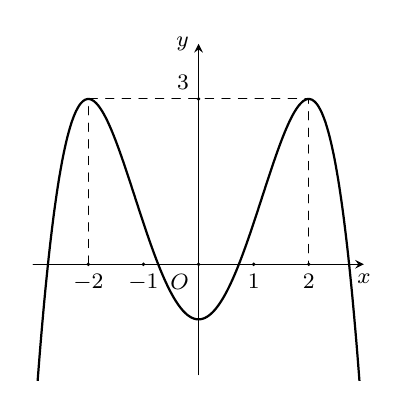
\begin{tikzpicture}[scale=.7, font=\footnotesize, line join=round, line cap=round,>=stealth]
		\def\xmin{-3};\def\ymin{-2};\def\xmax{3};\def\ymax{4};
		\coordinate (O) at (0,0);
		\draw[->] (\xmin,0)--(\xmax,0) node[below]{$x$};
		\draw[->] (0,\ymin)--(0,\ymax) node[left]{$y$};
		\fill (O) node[below left]{$O$} circle(1pt);
		\clip ({\xmin-0.1},{\ymin-0.1}) rectangle ({\xmax+0.1},{\ymax+0.1});
		\foreach \x in {-2,-1,1,2}{\fill (\x,0) node[below]{$\x$} circle(1pt);}
		\foreach \y in {3}{\fill (0,\y) node[above left]{$\y$} circle(1pt);}
		\draw[thick,samples=100,smooth] plot[domain=-4:4](\x,{-1/4*(\x)^4+2*(\x)^2-1});
		\draw [dashed](-2,0)|-(0,3)-|(2,0);
	\end{tikzpicture}
	}
	\loigiai{
		Hàm số đã cho đồng biến trên khoảng $(-\infty;-2)$.
	}
\end{ex}
%%%==============EX_10============%%%
\begin{ex}%[2D1V1-2]
	\immini[thm]
	{Cho hàm số bậc bốn $y=f(x)$ có đồ thị là đường cong trong hình bên. Hàm số đã cho đồng biến trên khoảng nào dưới đây?
	\choice[2]
	{$(-5; 1)$}
	{\True  $(1;+\infty)$}
	{$(-\infty; 0)$}
	{$(-\infty; 5)$}}
	{
	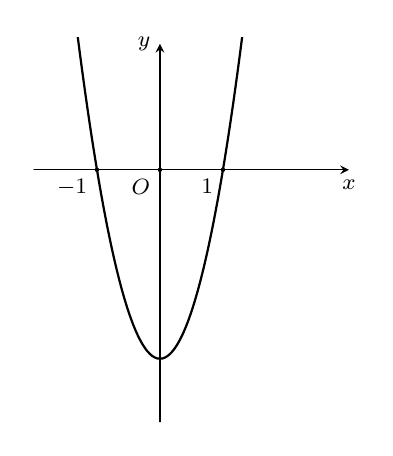
\begin{tikzpicture}[scale=.8, font=\footnotesize, line join=round, line cap=round,>=stealth]
		\def\xmin{-2};\def\ymin{-4};\def\xmax{3};\def\ymax{2};
		\coordinate (O) at (0,0);
		\draw[->] (\xmin,0)--(\xmax,0) node[below]{$x$};
		\draw[->] (0,\ymin)--(0,\ymax) node[left]{$y$};
		\fill (O) node[below left]{$O$} circle(1pt);
		\clip ({\xmin-0.1},{\ymin-0.1}) rectangle ({\xmax+0.1},{\ymax+0.1});
		\foreach \x in {-1,1}{\fill (\x,0) node[below left]{$\x$} circle(1pt);}
		\draw[thick,samples=100,smooth] plot[domain=-4:4](\x,{3*(\x)^2-3});
	\end{tikzpicture}
	}
	\loigiai{
		Hàm số đã cho đồng biến trên khoảng $(1;+\infty)$.
	}
\end{ex}
%%%==============EX_11============%%%
\begin{ex}%[2D1V1-2]
	\immini[thm]
	{Cho hàm số bậc bốn $y=f(x)$ có đồ thị là đường cong trong hình bên. Hàm số đã cho đồng biến trên khoảng nào dưới đây?
	\choice[2]
	{$(4;+\infty)$}
	{$(-2; 3)$}
	{$(-2; 0)$}
	{\True $(-\infty;-5)$}}
	{
		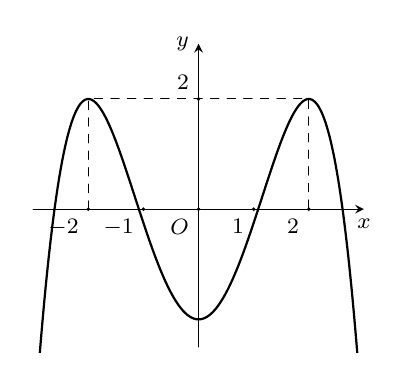
\begin{tikzpicture}[scale=.7, font=\footnotesize, line join=round, line cap=round,>=stealth]
		\def\xmin{-3};\def\ymin{-2.5};\def\xmax{3};\def\ymax{3};
		\coordinate (O) at (0,0);
		\draw[->] (\xmin,0)--(\xmax,0) node[below]{$x$};
		\draw[->] (0,\ymin)--(0,\ymax) node[left]{$y$};
		\fill (O) node[below left]{$O$} circle(1pt);
		\clip ({\xmin-0.1},{\ymin-0.1}) rectangle ({\xmax+0.1},{\ymax+0.1});
		\foreach \x in {-2,-1,1,2}{\fill (\x,0) node[below left]{$\x$} circle(1pt);}
		\foreach \y in {2}{\fill (0,\y) node[above left]{$\y$} circle(1pt);}
		\draw[thick,samples=100,smooth] plot[domain=-4:4](\x,{-1/4*(\x)^4+2*(\x)^2-2});
		\draw [dashed](-2,0)|-(0,2)-|(2,0);
	\end{tikzpicture}
	}
	\loigiai{
		Hàm số đã cho đồng biến trên khoảng $(-\infty;-5)$.
	}
\end{ex}
%%%==============EX_12============%%%
\begin{ex}%[2D1V1-2]
	\immini[thm]
	{Cho hàm số bậc bốn $y=f(x)$ có đồ thị là đường cong trong hình bên. Hàm số đã cho đồng biến trên khoảng nào dưới đây?
	\choice[2]
	{$(-\infty; 3)$}
	{$(-\infty; 0)$}
	{\True $(3;+\infty)$}
	{$(-2; 2)$}}
	{
		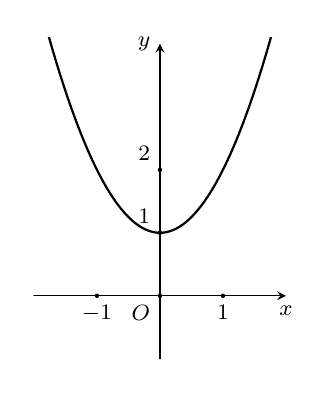
\begin{tikzpicture}[scale=.8, font=\footnotesize, line join=round, line cap=round,>=stealth]
		\def\xmin{-2};\def\ymin{-1};\def\xmax{2};\def\ymax{4};
		\coordinate (O) at (0,0);
		\draw[->] (\xmin,0)--(\xmax,0) node[below]{$x$};
		\draw[->] (0,\ymin)--(0,\ymax) node[left]{$y$};
		\fill (O) node[below left]{$O$} circle(1pt);
		\clip ({\xmin-0.1},{\ymin-0.1}) rectangle ({\xmax+0.1},{\ymax+0.1});
		\foreach \x in {-1,1}{\fill (\x,0) node[below]{$\x$} circle(1pt);}
		\foreach \y in {1,2}{\fill (0,\y) node[above left]{$\y$} circle(1pt);}
		\draw[thick,samples=100,smooth] plot[domain=-4:4](\x,{(\x)^2+1});
	\end{tikzpicture}
	}
	\loigiai{
		Hàm số đã cho đồng biến trên khoảng $(3;+\infty)$.
	}
\end{ex}
\Closesolutionfile{ans}
\indapan{6}{ans/ans-2-B1-De1}
\cauds
\Opensolutionfile{ans}[ans/ans-2-B1-De1-DS]
%%%%==============EX_13============%%%
\begin{ex}%[2D1V1-1]
	Cho hàm số $y=f(x)=x^3-3x^2+2$. Các khẳng định dưới đây đúng hay sai?
	\choiceTF
	 {Hàm số đồng biến trên khoảng $(-\infty; 2)$}
	 {Hàm số đồng biến trên khoảng $(2;+\infty)$}
	 {Hàm số đạt cực tiểu tại điểm $x=2$}
	 {Giá trị $y_{\text{CĐ}}^2+y_{CT}^2$ bằng $8$}
\loigiai{
	Ta có $f'(x)=3x^2-6x \Rightarrow f'(x)=0\Leftrightarrow \hoac{&x=0\\ &x=2.}$\\
	Ta có bảng biến thiên
\begin{center}
	
\begin{tikzpicture}
		\tkzTabInit[nocadre=false,lgt=2,espcl=2,deltacl=0.5]
		{$x$/1 , $f'(x)$/1 , $f(x)$/2}
		{$-\infty$,$0$,$2$,$+\infty$}
		\tkzTabLine{,+,0,-,0,+,}
		\tkzTabVar{-/$-\infty$,+/$2$,-/$-2$,+/$+\infty$}
	\end{tikzpicture}
\end{center}
\begin{itemchoice}
	\itemch Sai. Vì từ bảng biến thiên ta có hàm số đồng biến trên các khoảng $(-\infty; 0)$ và $(2;+\infty)$.
	\itemch Đúng. Hàm số đồng biến trên khoảng $(2;+\infty)$. 
	\itemch  Đúng. Hàm số đạt cực tiểu tại điểm $x=2$.
	\itemch Đúng. Vì  $y_{\text{CĐ}}=2, y_{CT}=-2 \Rightarrow y_{\text{CĐ}}^2+y_{CT}^2=8$. 
\end{itemchoice}
}
\end{ex}
%%%%==============EX_14============%%%
\begin{ex}%[2D1V1-1]
Cho hàm số $y=f(x)$ có bảng biến thiên
\begin{center}
	
\begin{tikzpicture}
		\tkzTabInit[nocadre=false,lgt=2,espcl=2,deltacl=0.5]
		{$x$/1 , $f'(x)$/1 , $f(x)$/2}
		{$-\infty$,$-1$,$0$,$1$,$+\infty$}
		\tkzTabLine{,-,+,0,-,0,+,}
		\tkzTabVar{+/$+\infty$,-/$-3$,+/$-2$,-/$-3$,+/$+\infty$}
	\end{tikzpicture}
\end{center}
\choiceTF
 {Hàm số nghịch biến trên khoảng $(-\infty;-1) \cup(0; 1)$}
 {Hàm số đồng biến trên khoảng $(2;+\infty)$}
 {Hàm số có $3$ điểm cực trị}
 {Giá trị $m^2\cdot y_{\text{CĐ}} +m\cdot y_{CT}+5=0$ khi và chỉ khi $\hoac{&m=1\\ &m=-\dfrac{5}{2}}$}
\loigiai{
 \begin{itemchoice}
 \itemch Sai. Vì hàm số $f(x)$ nghịch biến trên các khoảng $(-\infty;-1)$ và $(0; 1)$. 
 \itemch Đúng. Vì hàm số $f(x)$ đồng biến trên các khoảng $(-1; 0)$, $(1;+\infty) \Rightarrow$ hàm số đồng biến trên $(2;+\infty)$. 
 \itemch Đúng. Vì $f'(x)$ đổi dấu khi $x$ đi qua các điểm $-1$; $0$; $1$ nên hàm số $f(x)$ có ba điểm cực trị. 
 \itemch Đúng. Vì từ bảng biến thiên ta có \\
 $y_{\text{CĐ}}=-2$, $y_{CT}=-3 \Rightarrow-2 m^2-3 m+5=0 \Leftrightarrow\hoac{&m=1\\ &m=-\dfrac{5}{2}.}$
 \end{itemchoice}
}
\end{ex}
%%%%==============EX_15============%%%
\begin{ex}%[2D1V2-2]
	\immini
{Cho hàm số $y=f(x)$ có đồ thị như hình vẽ. 
\choiceTF
 {Hàm số nghịch biến trên khoảng $(0; 1)$}
 {Hàm số đạt cực đại tại $x=2$}
 {Hàm số có $3$ điểm cực trị}
 {Phương trình $f'(x)=0$ có ngiệm $x=0$ và $x=2$}}
 {
 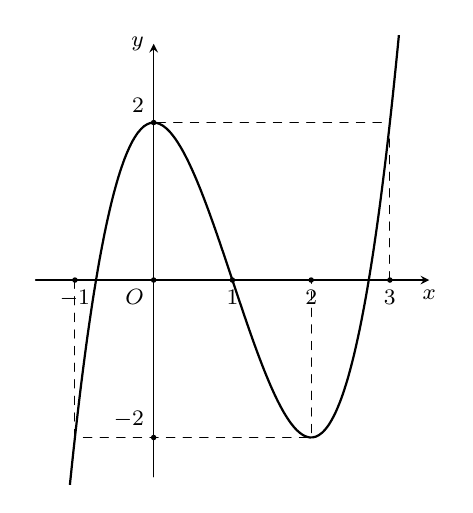
\begin{tikzpicture}[scale=1, font=\footnotesize, line join=round, line cap=round,>=stealth]
 	\def\xmin{-1.5};\def\ymin{-2.5};\def\xmax{3.5};\def\ymax{3};
 	\coordinate (O) at (0,0);
 	\draw[->] (\xmin,0)--(\xmax,0) node[below]{$x$};
 	\draw[->] (0,\ymin)--(0,\ymax) node[left]{$y$};
 	\fill (O) node[below left]{$O$} circle(1pt);
 	\clip ({\xmin-0.1},{\ymin-0.1}) rectangle ({\xmax+0.1},{\ymax+0.1});
 	\foreach \x in {-1,1,2,3}{\fill (\x,0) node[below]{$\x$} circle(1pt);}
 	\foreach \y in {-2,2}{\fill (0,\y) node[above left]{$\y$} circle(1pt);}
 	\draw[thick,samples=100,smooth] plot[domain=-4:4](\x,{(\x)^3-3*(\x)^2+2});
 	\draw [dashed] (-1,0)|-(0,-2)-|(2,0) (3,0)|-(0,2)
 	;
 \end{tikzpicture}
 }
\loigiai{
\begin{itemchoice}
\itemch Đúng. Vì từ đồ thị ta có hàm số $y=f(x)$ nghịch biến trên khoảng $(0; 2) \Rightarrow y=f(x)$ nghịch biến trên $(0; 1)$. 
\itemch Sai.  Vì từ đồ thị ta có hàm số đặt cực đại tại $x=0$. 
\itemch Sai. Vì hàm số $y=f(x)$ đạt cực đại tại $x=0$, cực tiểu tại $x=2$. 
\itemch Đúng. Vì hàm số $y=f(x)$ đạt cực đại tại $x=0$, cực tiểu tại $x=2$ nên phương trình $f'(x)=0$ có hai nghiệm $x=0, x=2$ hay $f'(x)=0 \Leftrightarrow \hoac{&x=0\\ &x=2.}$
\end{itemchoice}
}
\end{ex}
%%%%==============EX_16============%%%
\begin{ex}%[2D1V2-2]
Cho hàm số $y=f(x)$ xác định và liên tục trên $\mathbb{R}$. Hàm số $f'(x)$ có bảng xét dấu
\begin{center}
	
\begin{tikzpicture}
		\tkzTabInit[nocadre=false,lgt=2,espcl=2,deltacl=0.5]
		{$x$/1 , $f'(x)$/1}
		{$-\infty$,$-1$,$1$,$4$,$+\infty$}
		\tkzTabLine{,-,0,+,0,-,0,+,}
	\end{tikzpicture}
\end{center}
\choiceTF
{Hàm số đồng biến trên khoảng $(0; 1)$}
{Hàm số đạt cực đại tại $x=4$}
{Hàm số có $3$ điểm cực trị}
{Hàm số $g(x)=f(1-x)$ đồng biến trên khoảng $(-3; 0)$}
\loigiai{
\begin{itemchoice}
\itemch Đúng. Vì hàm số $y=f(x)$ đồng biến trên khoảng $(-1; 1) \Rightarrow y=f(x)$ đồng biến trên $(0; 1)$. 
\itemch Sai. Vì từ đồ thị ta có hàm số đạt cực đại tại $x=1$. 
\itemch Đúng. Vì hàm số $y=f(x)$ có $3$ điểm cực trị. 
\itemch  Đúng. Vì ta có $g'(x)=-f'(1-x) \Rightarrow g'(x) > 0\Leftrightarrow-f'(1-x) > 0\Leftrightarrow f'(1-x) < 0$.\\
 Từ bảng xét dấu ta có
$f'(1-x) < 0\Leftrightarrow\hoac{&1-x <-1\\ &1< 1-x < 4} \Leftrightarrow\hoac{&x > 2\\&-3< x < 0.}$\\
Vậy hàm số $g(x)$ đồng biến trên các khoảng $(-3; 0)$ và $(2;+\infty)$.
\end{itemchoice}
}
\end{ex}
\Closesolutionfile{ans}
\indapan{3}{ans/ans-2-B1-De1-DS}
\caukq
\Opensolutionfile{ans}[ans/ans-2-B1-De1-KQ]
%%%%==============EX_17============%%%
\begin{ex}%[2D1V1-3]
Để hàm số $y=\dfrac{x^2+m x+1}{x+m}$ đạt cực đại tại $x=2$ thì $m=$?
\shortans{$-3$}
\loigiai{
Tập xác định $\mathscr{D}=\mathbb{R} \setminus \{-m\}$.\\
$y'=\dfrac{x^2+2m x+m^2-1}{(x+m)^2}$.\\ $y''=\dfrac{2}{(x+m)^3}$.\\
Hàm số đạt cực đại tại $x=2$ nên $\heva{&y'(2)=0\\ &y''(2) < 0} \Leftrightarrow\heva{&\dfrac{m^2+4m+3}{(m+2)^2}=0\\&\dfrac{2}{(m+2)^3} < 0} \Leftrightarrow m=-3$.
}
\end{ex}
%%%%==============EX_18============%%%
\begin{ex}%[2D1V2-6]
Đồ thị của hàm số $y=\dfrac{x^2-m x}{x+1}$ có hai điểm cực trị $A$, $B$ và $AB=5$ khi $m=$?
\shortans{$0{,}25$}
\loigiai{
Ta có $\mathscr{D}=\mathbb{R} \setminus\{-1\}$ và có đạo hàm là $y'=\dfrac{x^2+2x-m}{(x+1)^2}$.\\
Để hàm số có hai điểm cực trị ta phải có $\heva{&1+m > 0\\ &1-2-m \neq 0} \Leftrightarrow m >-1$.\\
Gọi hai hoành độ cực trị là $x_1$ và $x_2$ ta có $\heva{&x_1+x_2=-2\\ &x_1x_2=-m.}$\\
Khi đó điểm $A\left(x_1,2x_1-m\right)$ và $B\left(x_2,2x_2-m\right)$.\\
$AB=\sqrt{4+4m} \cdot \sqrt{5}=5\Leftrightarrow 4+4m=5\Leftrightarrow m=\dfrac{1}{4}=0{,}25$.
}
\end{ex}
%%%%==============EX_19============%%%
\begin{ex}%[2D1V1-3]
Có bao nhiêu giá trị nguyên của tham số $m$ để hàm số $y=\dfrac{x^2+2x+m}{x-1}$ nghịch biến trên khoảng $(1; 3)$ và đồng biến trên khoảng $(4; 6)$?
\shortans[]{$6$}
\loigiai{
Ta có $y'=\dfrac{x^2-2x-2-m}{(x-1)^2}$.
Hàm số nghịch biến trên khoảng $(1; 3)$ và đồng biến trên khoảng $(4; 6)$ khi và chỉ khi\\
	$\heva{&y' \leq 0, \forall x \in(1; 3) \\
		&y' \geq 0, \forall x \in(4; 6)
		&} \Leftrightarrow\heva {x ^ {2}-2x-2-m \leq 0, \forall x \in (1; 3)\\
		x ^ {2}-2x-2-m \geq 0, \forall x \in (4; 6)} $\\
		$\Leftrightarrow \heva{&m \geq x^2-2x-2, \forall x \in(1; 3) \\
		&m \leq x^2-2x-2, \forall x \in(4; 6).}$\\
Xét hàm số $g(x)=x^2-2x-2, g'(x)=2x-2$ ta có bảng biến thiên của $g(x)$ như sau
\begin{center}
	\begin{tikzpicture}
		\tkzTabInit[nocadre=true,lgt=1.2,espcl=3,deltacl=0.6]
		{$x$ /0.6,$g'(x)$ /0.6,$g(x)$ /4.0}
		{$-\infty$,$1$,$3$,$4$,$6$,$+\infty$}
		\tkzTabLine{,-,$0$,+,|,+,|,+,|,+,}		
		\path
		(N11)--(N13)node(N1)[pos=0.2]{$+\infty$}
		(N21)--(N23)node(N2)[pos=0.9]{$-3$}
		(N32)--(N33)node(N3)[pos=0.7]{$1$}
		(N41)--(N43)node(N4)[pos=0.55]{$6$}
		(N51)--(N53)node(N5)[pos=0.35]{$18$}
		(N61)--(N63)node(N6)[pos=0.2]{$+\infty $}					
		;		
		\foreach \a/\b in {1/2,2/3,3/4,4/5,5/6}
		\draw[line width=1,blue,->] (N\a)--(N\b);
		
	\end{tikzpicture}
\end{center}
Từ bảng biến thiên của $g(x)$ ta có $(*) \Leftrightarrow 1\leq m \leq 6$, và vì $m$ là số nguyên nên chọn $m \in\{1; 2; 3; 4; 5; 6\}$. \\
Vậy có $6$ giá trị nguyên của $m$ thỏa mãn bài toán.
}
\end{ex}
%%%%==============EX_20============%%%
\begin{ex}%[2D1V3-6]
Một doanh nghiệp dự kiến lợi nhuận khi sản xuất $x$ sản phẩm $(0\leq x \leq 300)$ được cho bởi hàm số $y=-x^3+300x^2$ (đơn vị: đồng). Hỏi doanh nghiệp cần sản xuất bao nhiêu sản phẩm để đạt được lợi nhuận cao nhất?
\shortans{$200$}
\loigiai{
Xét hàm số $y=-x^3+300x^2$ trên đoạn $[0; 300]$.\\
$y'=-3x^2+600x$.\\
$y'=0\Leftrightarrow-3x^2+600x=0\Leftrightarrow\hoac{&x=0\\ &x=200.}$\\
Bảng biến thiên
		\begin{center}
	
\begin{tikzpicture}
		\tkzTabInit[nocadre=false,lgt=2,espcl=2,deltacl=0.5]
		{$x$/1 , $f'(x)$/1 , $f(x)$/2}
		{$-\infty$,$0$,$200$,$+\infty$}
		\tkzTabLine{,-,0,+,0,-,}
		\tkzTabVar{+/$+\infty$,-/$0$,+/$4\,000\,000$,-/$-\infty$}
	\end{tikzpicture}
\end{center}
Từ bảng biến thiên suy ra lợi nhuận cao nhất khi số sản phẩm sản xuất là $200$ sản phẩm.
}
\end{ex}
%%%%============EX_21==============%%%
\begin{ex}%[2D1V3-6]
Kính viễn vọng không gian Hubble được đưa vào vũ trụ ngày 24/4/1990 bằng tàu con thoi Discovery. Vận tốc của tàu con thoi trong sứ mệnh này, từ lúc cất cánh tại thời điểm $t=0$ (s) cho đến khi tên lửa đẩy được phóng đi tại thời điểm $t=126$ (s), cho bởi hàm số sau $v(t)=0{,}001302t^3-0{,}09029t^2+23$ ($v$ được tính bằng ft/s, $1$ feet $=0{,}3048$ m)~ (\textit{Nguồn: J. Stewart, Calculus, Seventh Edition, Brooks/Cole, CENGAGE Learning 2012}).
Hỏi số nguyên nhỏ nhất $t$ để gia tốc của tàu con thoi tăng trong khoảng thời gian tính từ thời điểm cất cánh cho đến khi tên lửa đẩy được phóng đi là bao nhiêu?
\shortans{$24$}
\loigiai{
Gia tốc của tàu con thoi $a(t)=0{,}003906t^2-0{,}18058t$ trên đoạn $[0; 126]$.\\
$a'(t)=0,007812t-0,18058$.\\
$a'(t)=0\Leftrightarrow 0{,}007812t-0{,}18058=0\Leftrightarrow t \approx 23{,}12$.\\
Bảng biến thiên
\begin{center}
	
\begin{tikzpicture}[>=stealth]
		\tkzTabInit[nocadre=false,lgt=1,espcl=3,deltacl=0.5]{$x$/.7 ,$y'$/.7,$y$/2}
		{$-\infty$ , $23{,}12$ , $+\infty$}
		\tkzTabLine{ , - , $0$ , + , }
		\tkzTabVar{+/$+\infty$ , -/$-2{,}1$ , +/$+\infty$}
	\end{tikzpicture}
\end{center}
Từ bảng biến thiên suy ra gia tốc của tàu con thoi sẽ tăng sau $t \approx 23{,}12$ (s).}
\end{ex}
%%%%==============EX_22============%%%
\begin{ex}%[2D1V3-6]%[2H2N1-1]
Khi loại thuốc A được tiêm vào bệnh nhân, nồng độ mg/l của thuốc trong máu sau $x$ phút (kể từ khi bắt đầu tiêm) được xác định bởi công thức $C(x)=\dfrac{30x}{x^2+2}$
(\textit{Nguồn: James Stewart, J. (2015). Calculus. Cengage Learning}). Để đưa ra những lời khuyên và cách xử lí phù hợp cho bệnh nhân, ta cần tìm khoảng thời gian mà nồng độ của thuốc trong máu đang tăng. Em hãy cho biết hàm nồng độ
thuốc trong máu $C(x)$ đạt giá trị cực đại là bao nhiêu trong khoảng thời gian $6$ phút sau khi tiêm (kết quả làm tròn đến hang phần mười)?
\shortans{$10{,}6$}
\loigiai{
Xét hàm số $y=C(x)=\dfrac{30x}{x^2+2}$ trên khoảng $(0;+\infty)$.\\
$y'=\dfrac{-30x^2+60}{\left(x^2+2\right)^2}$.\\
$y'=0\Leftrightarrow \dfrac{-30x^2+60}{\left(x^2+2\right)^2}=0\Leftrightarrow\hoac{&x=\sqrt{2}&(\text{nhận}) \\ &x=-\sqrt{2}&(\text{loại}).}$\\
Bảng biến thiên
\begin{center}
		
\begin{tikzpicture}
		\tkzTabInit[nocadre=false,lgt=2,espcl=3,deltacl=0.5]
		{$x$/1 , $f'(x)$/1 , $f(x)$/2}
		{$-\infty$,$-\sqrt{2}$,$\sqrt{2}$,$+\infty$}
		\tkzTabLine{,-,0,+,0,-,}
		\tkzTabVar{+/$+\infty$,-/$-\dfrac{15\sqrt{2}}{2}$,+/$\dfrac{15\sqrt{2}}{2}$,-/$-\infty$}
	\end{tikzpicture}
\end{center}
Từ bảng biến thiên suy ra nồng độ thuốc trong máu $C(x)$ đạt giá trị cực đại là $\dfrac{15\sqrt{2}}{2}$ mg/l trong khoảng thời gian $6$ phút sau khi tiêm.
}
\end{ex}
\Closesolutionfile{ans}
\indapan{6}{ans/ans-2-B1-De1-KQ}